%0       1         2         3         4         5         6         7         8
%2345678901234567890123456789012345678901234567890123456789012345678901234567890
%=======================================================================
\documentclass{article}
%=======================================================================


% INCLUDE DEVELOPMENT TEXT

\newcommand{\devel}[1]{\textbf{#1}}

% EXCLUDE DEVELOPMENT TEXT

% \newcommand{\devel}[1]{}


%=======================================================================
% Document layout
%=======================================================================

\setlength{\topmargin}{0.0in}
\setlength{\oddsidemargin}{0.0in}
\setlength{\evensidemargin}{0.0in}
\setlength{\textwidth}{6.0in}
\setlength{\textheight}{9.0in}

%=======================================================================
% Packages
%=======================================================================

\usepackage{wasysym}
\usepackage{epsfig}
\usepackage{url}

%=======================================================================
% Commands
%=======================================================================

\newcommand{\cello}{\textsf{Cello}}
\newcommand{\enzo}{\textsf{Enzo}}
\newcommand{\lcaperf}{\textsf{lcaperf}}
\newcommand{\lcatest}{\textsf{lcatest}}

\newcommand{\code}[1]{\textsf{#1}}

\newcommand{\note}[1]{\devel{\eighthnote\ \textit{#1} \\}}
\newcommand{\pargraph}[1]{\devel{\P\ \textbf{#1} \\}}

\newcommand{\todo}{\devel{$\circ$}}
\newcommand{\done}{\devel{$\bullet$}}
\newcommand{\halfdone}{\devel{\textcolor{gray}{$\bullet$}}}

\newcommand{\PROJECT}{\cello}

\newcommand{\TITLE}[3]{
\title{ {\huge \PROJECT\ #1}  \\ \vspace{0.1in}
     {\small Document Version: \textbf{#3}} \vspace{-0.1in}
    }
\author{      #2 \\
        Laboratory for Computational Astrophysics\\
        University of California, San Diego}
\maketitle}

%=======================================================================


%=======================================================================

\begin{document}

%=======================================================================
\TITLE{Software Design Description}{James Bordner}{unigrid hydro}
%=======================================================================

\tableofcontents
%=======================================================================
\section{Introduction} \label{s:intro}
%=======================================================================

Computer languages used will be C++, C99, and source languages of
incorporated legacy code.  Parallelism support will include MPI-1
two-sided communication (send/receive), MPI-2's one-sided
communication (\code{get()}), UPC, and OpenMP.

%=======================================================================
\section{Compilation configuration} \label{s:compile}
%=======================================================================

%=======================================================================
\section{Command-line options} \label{s:commandline}
%=======================================================================

Usage: \code{cello} \textit{parameter-file}

%=======================================================================
\section{Components} \label{s:components}
%=======================================================================

\begin{itemize}
\item Control
\item Problem
\item Method
\item Data
\item Parallel
\item IO
\end{itemize}


%=======================================================================
\section{Input parameters} \label{s:input}
%=======================================================================

\cello\ is controlled by parameters specified in an input file.  Parameters
are organized into the following categories:

\begin{itemize}
\item Problem
\item Physics
\item Algorithms
\item Data
\item Parallel
\item I/O
\item Performance
\end{itemize}

Equivalent \enzo\ parameters

\begin{tabular}{ll}
ControlCourantSafetyFactor        & CourantSafetyNumber \\
ControlStopCycle           & StopCycle \\
ControlStopTime            & StopTime \\
HydroMethod                & HydroMethod \\
HydroParameter "diffusion"    & PPMDiffusionParameter \\
HydroParameter "dual-energy"  & DualEnergyFormalism \\
HydroParameter "eta1"    & DualEnergyFormalismEta1 \\
HydroParameter "eta2"    & DualEnergyFormalismEta2 \\
HydroParameter "flattening"   & PPMFlatteningParameter \\
HydroParameter "pressure free" & PressureFree \\
HydroParameter "steepening"  & PPMSteepeningParameter \\
Material1Gamma             & Gamma \\
OutputUserDt               & dtDataDump \\
OutputUserDumpName         & DataDumpName \\
ProblemBcLower             & LeftFaceBoundaryCondition \\
ProblemBcUpper             & RightFaceBoundaryCondition \\
ProblemDomainLower         & DomainLeftEdge \\
ProblemDomainUpper         & DomainRightEdge \\
ProblemStartCycle          & InitialCycleNumber \\
ProblemStartTime           & InitialTime \\
                           & ProblemType \\
\end{tabular}

%-----------------------------------------------------------------------
\subsection{Problem parameters}
%-----------------------------------------------------------------------

Problem parameters specify the setup of the physical problem,
including initial conditions of relevant data fields and boundary
conditions.

  dimensionality
  domain extents
  initial conditions (materials, regions, input)
 boundary conditions (periodic, in-/out-flow, specified, dynamic)

%-----------------------------------------------------------------------
\subsection{Physics parameters}
%-----------------------------------------------------------------------

Physics parameters specify physics modules and units.

 hydrodynamics
  cosmological expansion
 self-gravity

Hydrodynamics


%-----------------------------------------------------------------------
\subsection{Algorithms parameters} 
%-----------------------------------------------------------------------

Specify algorithms and their parameters.

Hydrodynamics dual-energy

Hydrodynamics steepening
Hydrodynamics flattening
Hydrodynamics diffusion

Timestepping

%-----------------------------------------------------------------------
\subsection{Data parameters}
%-----------------------------------------------------------------------

Specify low-level datastructures (fields and particles) and their
parameters.

Use chunked field storage \\
Field chunk size or range

%-----------------------------------------------------------------------
\subsection{Parallel parameters}  \label{ss:parallel}
%-----------------------------------------------------------------------

Specifiy method for controling parallelism

   parallelization method (MPI buffered/blocking, MPI2 Get)


%-----------------------------------------------------------------------
\subsection{I/O parameters} 
%-----------------------------------------------------------------------

Output types and parameters
 checkpoint (dump all)
 output (specific fields)
 movies (type and rate)
 analysis (type of analysis, rate)
 level of output (files for timestep, time, etc.)


%-----------------------------------------------------------------------
\subsection{Performance parameters} 
%-----------------------------------------------------------------------

Performanec parameters control \lcaperf\ instrumentation.



%=======================================================================
\section{Classes} \label{s:classes}
%=======================================================================

\begin{tabbing}
xxx\=xxx\=xxx\=xxx\=xxxxxxxx\= \kill
 \>      \code{Control}     \>\>\>\> \textit{Manages everything}  \\
 \>\>    \code{Parameters}    \>\>\> \textit{Reading and accessing all parametrs} \\
 \>\>    \code{Parallel}      \>\>\> \textit{Manages multiple parallelization levels and technologies} \\
 \>\>    \code{Recovery}      \>\>\> \textit{Detects, evaluates, and recovers from hardware or software errors} \\
 \>\>    \code{Portal}        \>\>\> \textit{Controls access to internal state and data by external entities} \\
 \>\>    \code{Performance}   \>\>\> \textit{Measures and allows other components to access performance data} \\
 \>\>    \code{Monitor}       \>\>\> \textit{Enables users to monitor the state and progress of the simulations} \\
 \>      \code{Simulation}  \>\>\>\> \textit{Description of a single astrophysics simulation} \\
 \>\>    \code{Problem}       \>\>\> \textit{Declaration of what to simulation} \\
 \>\>\>  \code{Domain}          \>\> \textit{The problem domain} \\
 \>\>\>  \code{Field}           \>\> \textit{A scalar or vector field} \\
 \>\>\>  \code{Boundary}        \>\> \textit{Boundary conditions} \\
 \>\>\>  \code{Initial}         \>\> \textit{Initial conditions} \\
 \>\>\>\>\code{Region}            \> \textit{A subset of the domain} \\
 \>\>    \code{Physics}       \>\>\> \textit{A physical law or process and associated parameters} \\
 \>\>\>  \code{Units}           \>\> \textit{Units used for user and computational fields} \\
 \>\>\>  \code{Material}        \>\> \textit{Type of matter, e.g.~gas, H+, e-, dark matter} \\
 \>\>    \code{Method}        \>\>\> \textit{Numerical method for evolving a physical law or laws} \\
 \>\>    \code{Analysis}      \>\>\> \textit{Numerical method for post-processing data} \\
 \>\>    \code{Data}          \>\>\> \textit{Numerical representation of data fields} \\
 \>\>\>  \code{Hierarchy}       \>\> \textit{AMR hierarchy} \\
 \>\>\>  \code{Level}           \>\> \textit{Uniform resolution component of an AMR hierarchy} \\
 \>\>\>  \code{Patch}           \>\> \textit{Rectangular grid of cells of uniform resolution in a hierarchy} \\
 \>\>\>\>\code{Box}               \> \textit{Rectangular box with position and size} \\
 \>\>\>\>\code{Array}             \> \textit{Array of floating-point values} \\
 \>\>\code{Output}            \>\>\> \textit{Description of what data to output, how, and when}
\end{tabbing}


%=======================================================================
\section{Problem Classes} \label{s:problem-classes}
%=======================================================================

%-----------------------------------------------------------------------
\subsection{\code{Simulation} class}
%-----------------------------------------------------------------------

The \code{Simulation} class is used to define a simulation.  
\begin{itemize}
\item \code{Problem}
\end{itemize}

\textbf{Attributes.}

\subsubsection{Operations}

%-----------------------------------------------------------------------
\subsection{\code{Parameters} class}
%-----------------------------------------------------------------------

The \code{Parameters} class read in a parameter file or files, and
provide the application access to parameter values.


\subsubsection{Attributes}

\subsubsection{Operations}

%-----------------------------------------------------------------------
\subsection{\code{Physics} class}
%-----------------------------------------------------------------------


\subsubsection{Attributes}

\subsubsection{Operations}

%-----------------------------------------------------------------------
\subsection{\code{Domain} class}
%-----------------------------------------------------------------------

The \code{Domain} class defines the problem domain


\subsubsection{Attributes}

\subsubsection{Operations}

%-----------------------------------------------------------------------
\subsection{\code{BC} class}
%-----------------------------------------------------------------------

The \code{BC} class defines boundary conditions on a \code{Domain}.



\subsubsection{Attributes}

\subsubsection{Operations}

%-----------------------------------------------------------------------
\subsection{\code{IC} class}
%-----------------------------------------------------------------------

The \code{IC} class defines initial conditions for a set of
\code{Field}s in a \code{Domain}.


\subsubsection{Attributes}

\subsubsection{Operations}

%-----------------------------------------------------------------------
\subsection{\code{Problem} class}
%-----------------------------------------------------------------------

The \code{Problem} class defines the problem to be solved, including
the domain, boundary conditions, and initial field values.


\subsubsection{Attributes}

\subsubsection{Operations}

%-----------------------------------------------------------------------
\subsection{\code{Field} class} \label{ss:field}
%-----------------------------------------------------------------------

A \code{Field} represents a discrete multiresolution scalar or vector
field.  A \code{Field} is associated with a \code{Hierarchy}, and is
composed of \code{Array}'s defined on a subset of \code{Grid}s in the
\code{Hierarchy}.

\subsubsection{Attributes}

\subsubsection{Operations}

%-----------------------------------------------------------------------
\subsection{\code{Units} class}
%-----------------------------------------------------------------------

A \code{Units} class represents the physical units for the data in a
\code{Field}.

\subsubsection{Attributes}

\subsubsection{Operations}

\newpage

%=======================================================================
\section{Data Classes} \label{s:data-classes}
%=======================================================================

\centerline{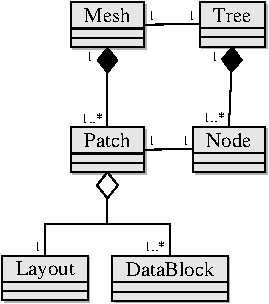
\includegraphics{uml/amr.1}}

%-----------------------------------------------------------------------
\subsection{\code{Hierarchy} class}
%-----------------------------------------------------------------------

A \code{Hierarchy} class represents a distributed structured AMR grid
hierarchy.  A \code{Hierarchy} can be considered to be an aggregate of
\code{Level}s, each of which in turn is an aggregate of individual
\code{Patch}es.  A patch is composed of a \code{Box}, which defines
the position and size in space, and some number of \code{Array}s, which
are used to store \code{Field} data (see \S\ref{ss:field}).



\subsubsection{Attributes}

\subsubsection{Operations}

%-----------------------------------------------------------------------
\subsection{\code{Level} class}
%-----------------------------------------------------------------------

A \code{Level} class represents a level in a distributed structured
AMR grid hierarchy (\code{Hierarchy}, where a level is defined as all
grid patches (\code{Grid}s) that have the same resolution.  A
\code{Level} is usually contained in a \code{Hierarchy}.

% The AMR hierarchy is represented using the trio of classes
% \code{Hierarchy}, \code{Level}, and \code{Grid}.
%   A \code{Grid} is a
% box in space, and is decomposed into \code{GridLocal} and
% \code{GridRemote} classes (see \S\ref{sss:class-grid}).  Each
% \code{GridLocal} object has some number of \code{Field} objects
% associated with them (see \S\ref{sss:class-field}), though the
% \code{GridLocal} objects themselves do not store field data
% themselves.  A \code{Level} class is also either a ``structured''
% \code{LevelStruct} or an ``unstructured'' \code{LevelUnstruct}.
% Structured levels are composed of a regular array of \code{Grid}s, and
% is typically used for unigrid calculations or the root level of an AMR
% calculation.  Unstructured levels are typically used for non-root
% levels of an AMR calulation.

\subsubsection{Attributes}

\subsubsection{Operations}

%-----------------------------------------------------------------------
\subsection{\code{Patch} class}
%-----------------------------------------------------------------------

A \code{Patch} class represents a grid patch in a distributed structured
AMR grid hierarchy (\code{Hierarchy}).  A \code{Patch} is defined by a
\code{Box}, and a set of \code{Array}s defined on the \code{Patch}.  Each
\code{Patch} is contained within a \code{Level}, and may be distributed
according to a \code{Parallel} object \S\ref{ss:parallel}.

\subsubsection{Attributes}

\subsubsection{Operations}

%-----------------------------------------------------------------------
\subsection{\code{Box} class}
%-----------------------------------------------------------------------

The \code{Box} class is for representing a box, and provides KeLP-like functionality.
Boxes are determined by two points, which may be of any parameterized type
(e.g.~\code{int} or \code{double}, etc.).


\subsubsection{Attributes}

\subsubsection{Operations}

%-----------------------------------------------------------------------
\subsection{\code{Array} class}
%-----------------------------------------------------------------------

The \code{Array} class encapsulates Fortran-style arrays with
convenient operations.  \code{Array}s may have optional support for
storing blocked or chunked arrays, include array padding, or store
interleaved arrays.  Arrays may be parallelized according to an
associated (static?) \code{Parallel} object (\S\ref{ss:parallel}).

% \centerline{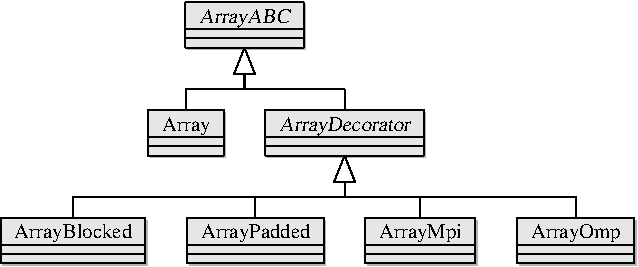
\includegraphics{uml/arrays.1}}

% \centerline{\includegraphics{uml/arrayabc.1}}

\centerline{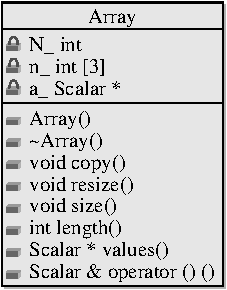
\includegraphics{uml/array.1}}

\textbf{Array shape.}

\textbf{Array blocking.}

\textbf{Array padding.}

\textbf{Array interleaving.}


\subsubsection{Attributes}

\begin{tabbing}
xx\=xx\=xxxxxxxxxxxxxxxxxxxxxxxxxxxxxxxxxxx\= \kill
\> \todo \>  \textit{Length of the allocated array} \\
\>       \> \code{N\_: int }      \\ \\
\> \todo \>  \textit {The shape of the array} \\
\>       \> \code{n\_: int [4] }  \\ \\
\> \todo \>  \textit {The array values, stored in column major ordering}\\
\>       \> \code{a\_: Scalar * }
\end{tabbing}

\subsubsection{Operations}

\begin{tabbing}
xx\=xx\=xxxxxxxxxxxxxxxxxxxxxxxxxxxxxxxxxxx\= \kill
\> \todo \> \textit{Create an uninitialized array} \\
\>       \> \code{Array()} \\ \\
\> \todo \> \textit{Create an initialized array of up to 4 dimensions} \\
\>       \> \code{Array(int n0, int n1=1, int n2=1, int n3=1)} \\ \\
\> \todo \> \textit{Delete and deallocate the array} \\
\>       \> \code{\~{\ }Array()}  \\ \\
\> \todo \> \textit{Copy an existing array} \\
\>       \> \code{void copy (const Array \&)}  \\ \\
\> \todo \> \textit{Reallocates the array with given shape.  All existing valuesare lost.} \\
\>       \> \code{void resize (int n0, int n1=1, int n2=1, int n3=1)}   \\ \\
\> \todo \> \textit{Get the extents of the array} \\
\>       \> \code{void size (int *n0, int *n1=0, int *n2=0, int *n3=0) const}  \\ \\
\> \todo \> \textit{Return the length of the array} \\
\>       \> \code{int length () const}  \\ \\
\> \todo \> \textit{Return a pointer to the array values (dangling pointer hazzard!)} \\
\>       \> \code{Scalar * values () const}  \\ \\
\> \todo \> \textit{Return the specified array element} \\
\>       \> \code{Scalar \& operator () (int i0, int i1=0, int i2=0, int i3=0)}
\end{tabbing}
%==================================================================
\end{document}
%==================================================================

